\documentclass[a4paper,12pt]{article}

% ======================================================================
% PACKAGES
% ======================================================================
\usepackage[utf8]{inputenc}
\usepackage[T1]{fontenc}
\usepackage{amsmath,amssymb}
\usepackage{array}
\usepackage{booktabs}
\usepackage{geometry}
\usepackage{parskip}
\usepackage{enumitem}
\usepackage{caption}
\usepackage{hyperref}
\usepackage{tabularx}
\usepackage{multirow}
\usepackage{xcolor}
\usepackage[most]{tcolorbox}
\usepackage{float}
\usepackage{siunitx}
\usepackage{graphicx}
\usepackage{tikz}
\usetikzlibrary{arrows.meta,positioning,shapes.geometric,calc}

\geometry{margin=2.5cm}

\hypersetup{
    colorlinks=true,
    linkcolor=blue!60!black,
    urlcolor=blue!60!black,
    citecolor=blue!60!black
}

\setlist[itemize]{topsep=3pt,itemsep=2pt,parsep=0pt}
\setlist[enumerate]{topsep=3pt,itemsep=2pt,parsep=0pt}
\captionsetup{font=small,labelfont=bf}

\newcolumntype{Y}{>{\raggedright\arraybackslash}X}

% ======================================================================
% BOX STYLES
% ======================================================================
\newtcolorbox{notebox}[1][]{
    enhanced,
    colback=blue!4!white,
    colframe=blue!55!black,
    fonttitle=\bfseries,
    title=#1,
    boxrule=0.6pt,
    arc=2mm,
    left=2mm,right=2mm,top=1mm,bottom=1mm
}

\newtcolorbox{warnbox}[1][]{
    enhanced,
    colback=orange!5!white,
    colframe=orange!65!black,
    fonttitle=\bfseries,
    title=#1,
    boxrule=0.6pt,
    arc=2mm,
    left=2mm,right=2mm,top=1mm,bottom=1mm
}

\newtcolorbox{keybox}[1][]{
    enhanced,
    colback=green!4!white,
    colframe=green!45!black,
    fonttitle=\bfseries,
    title=#1,
    boxrule=0.6pt,
    arc=2mm,
    left=2mm,right=2mm,top=1mm,bottom=1mm
}

\newtcolorbox{calcbox}[1][]{
    enhanced,
    colback=purple!4!white,
    colframe=purple!55!black,
    fonttitle=\bfseries,
    title=#1,
    boxrule=0.6pt,
    arc=2mm,
    left=2mm,right=2mm,top=1mm,bottom=1mm
}

\newtcolorbox{errbox}[1][]{
    enhanced,
    colback=red!4!white,
    colframe=red!60!black,
    fonttitle=\bfseries,
    title=#1,
    boxrule=0.6pt,
    arc=2mm,
    left=2mm,right=2mm,top=1mm,bottom=1mm
}

% ======================================================================
% TIKZ STYLES
% ======================================================================
\tikzset{
    workflowbox/.style={
        rectangle,
        rounded corners,
        draw=#1!70!black,
        fill=#1!8!white,
        thick,
        align=center,
        text width=2.8cm,
        minimum height=1.65cm,
        inner sep=4pt
    },
    smallworkflowbox/.style={
        rectangle,
        rounded corners,
        draw=#1!70!black,
        fill=#1!8!white,
        thick,
        align=center,
        text width=2.65cm,
        minimum height=1.45cm,
        inner sep=3pt
    },
    workflowarrow/.style={
        -{Latex[length=2mm]},
        thick,
        draw=black!65
    },
    feedbackarrow/.style={
        -{Latex[length=2mm]},
        thick,
        dashed,
        draw=black!55
    }
}

% ======================================================================
% TITLE
% ======================================================================
\title{\textbf{RSE3010: Mine Geotechnical Engineering}\\Week 4 Study Notes}
\author{Monash University, Semester 1, 2026}
\date{Based on Week 4 Lecture Slides}

\begin{document}

\maketitle

% ======================================================================
\section{Week 4: Deriving Design Parameters -- Rock Mass Failure Criteria}
% ======================================================================

\subsection{Purpose}

To derive rock mass strength and deformation parameters for engineering design using the
generalised Hoek--Brown failure criterion, while considering the influence of excavation
disturbance.

Two excavation scenarios are considered:
\begin{itemize}
    \item TBM excavation: low disturbance, \(D=0\);
    \item poor-quality drill-and-blast excavation: high disturbance, \(D=0.8\).
\end{itemize}

\begin{keybox}[Core idea]
Week 4 converts geological and laboratory information into engineering design parameters:
\[
\sigma_{ci},\ E_i,\ m_i,\ GSI,\ D
\quad \rightarrow \quad
m_b,\ s,\ a,\ \sigma_{cm},\ E_m,\ c,\ \phi
\]
These parameters are used in analytical calculations, empirical checks, and numerical
modelling.
\end{keybox}

% ======================================================================
\subsection{Learning Objectives}

By the end of this week, students should be able to:
\begin{itemize}
    \item apply the generalised Hoek--Brown criterion for jointed rock masses;
    \item explain the role of the disturbance factor \(D\);
    \item calculate rock mass Hoek--Brown parameters \(m_b\), \(s\), and \(a\);
    \item determine rock mass strength parameters, including \(\sigma_{cm}\), \(\sigma_{1m}^f\), and \(\sigma_{tm}\);
    \item estimate rock mass deformation modulus \(E_m\) using Hoek--Diederichs equations;
    \item convert the nonlinear Hoek--Brown envelope into equivalent Mohr--Coulomb parameters \(c\) and \(\phi\);
    \item distinguish between in-situ stress demand and failure-envelope strength capacity; and
    \item compare the influence of TBM and poor drill-and-blast excavation on design parameters.
\end{itemize}

% ======================================================================
\section{Where Week 4 Fits in the Design Chain}
% ======================================================================

\begin{figure}[H]
\centering
\resizebox{\textwidth}{!}{%
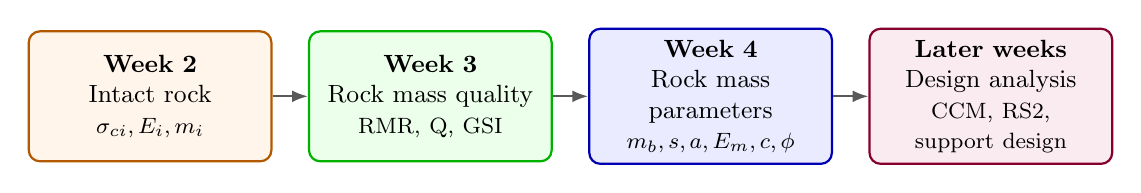
\begin{tikzpicture}[node distance=0.45cm, font=\small]

\node[workflowbox=orange] (w2)
{\textbf{Week 2}\\Intact rock\\
\footnotesize \(\sigma_{ci}, E_i, m_i\)};

\node[workflowbox=green, right=of w2] (w3)
{\textbf{Week 3}\\Rock mass quality\\
\footnotesize RMR, Q, GSI};

\node[workflowbox=blue, right=of w3] (w4)
{\textbf{Week 4}\\Rock mass parameters\\
\footnotesize \(m_b,s,a,E_m,c,\phi\)};

\node[workflowbox=purple, right=of w4] (future)
{\textbf{Later weeks}\\Design analysis\\
\footnotesize CCM, RS2, support design};

\draw[workflowarrow] (w2) -- (w3);
\draw[workflowarrow] (w3) -- (w4);
\draw[workflowarrow] (w4) -- (future);

\end{tikzpicture}
}
\caption{Week 4 converts intact rock data and GSI into rock mass design parameters.}
\label{fig:week4_design_chain}
\end{figure}

\begin{warnbox}[Why Week 4 is important]
Errors in \(GSI\), \(D\), or stress range selection can significantly change rock mass
strength, deformation modulus, and equivalent Mohr--Coulomb parameters. These errors
then propagate into later tunnel and cavern design calculations.
\end{warnbox}

% ======================================================================
\section{Generalised Hoek--Brown Criterion}
% ======================================================================

\subsection{Rock Mass Failure Criterion}

The generalised Hoek--Brown criterion for jointed rock masses is:
\[
\sigma_1^f =
\sigma_3 +
\sigma_{ci}
\left(
m_b\frac{\sigma_3}{\sigma_{ci}} + s
\right)^a
\]

where:
\begin{itemize}
    \item \(\sigma_1^f\) = major principal stress at failure;
    \item \(\sigma_3\) = confining stress used in the failure criterion;
    \item \(\sigma_{ci}\) = uniaxial compressive strength of intact rock;
    \item \(m_b\), \(s\), \(a\) = rock mass Hoek--Brown parameters;
    \item \(m_i\) = intact rock material constant;
    \item \(GSI\) = Geological Strength Index;
    \item \(D\) = disturbance factor.
\end{itemize}

\begin{keybox}[From intact rock to rock mass]
The intact Hoek--Brown criterion uses \(m_i\), \(s=1\), and \(a=0.5\).  
The generalised Hoek--Brown criterion modifies these values using \(GSI\) and \(D\)
to represent a jointed and disturbed rock mass.
\end{keybox}

% ----------------------------------------------------------------------
\subsection{Hoek--Brown Rock Mass Parameters}

The rock mass constants are calculated as:
\[
m_b =
m_i
\exp
\left(
\frac{GSI-100}{28-14D}
\right)
\]

\[
s =
\exp
\left(
\frac{GSI-100}{9-3D}
\right)
\]

\[
a =
\frac{1}{2}
+
\frac{1}{6}
\left(
e^{-GSI/15}
-
e^{-20/3}
\right)
\]

\begin{calcbox}[Key check]
For intact rock:
\[
GSI=100,\qquad D=0
\]
then:
\[
m_b=m_i,\qquad s=1,\qquad a=0.5
\]
and the criterion reduces to the original intact Hoek--Brown criterion.
\end{calcbox}

% ======================================================================
\section{Disturbance Factor \(D\)}
% ======================================================================

The disturbance factor accounts for blast damage, stress relaxation, and excavation-induced
disturbance around an opening. It reduces the rock mass strength and deformation modulus.

\begin{table}[H]
\centering
\small
\begin{tabularx}{\textwidth}{l Y c}
\toprule
\textbf{Excavation method} & \textbf{Description} & \textbf{Suggested \(D\)} \\
\midrule
TBM excavation & Mechanical excavation, minimal disturbance to surrounding rock & 0 \\
Good quality drill-and-blast & Controlled blasting, smooth wall, presplit & 0.5 \\
Poor quality drill-and-blast & Uncontrolled production blasting, significant damage & 0.8 \\
Very poor blasting & Heavy damage, stress relaxation & 1.0 \\
\bottomrule
\end{tabularx}
\caption{Typical disturbance factor \(D\) for different excavation methods.}
\label{tab:Dfactor}
\end{table}

\begin{warnbox}[Engineering effect of \(D\)]
Increasing \(D\) decreases \(m_b\), decreases \(s\), reduces rock mass strength, and reduces
rock mass modulus. Poor blasting can therefore significantly increase support demand even
when the original geological conditions are the same.
\end{warnbox}

% ======================================================================
\section{Week 4 Calculation Workflow}
% ======================================================================

\begin{figure}[H]
\centering
\resizebox{\textwidth}{!}{%
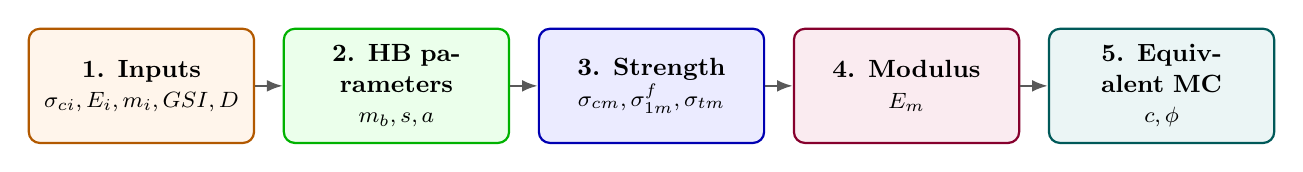
\begin{tikzpicture}[node distance=0.35cm, font=\small]

\node[smallworkflowbox=orange] (input)
{\textbf{1. Inputs}\\
\footnotesize \(\sigma_{ci},E_i,m_i,GSI,D\)};

\node[smallworkflowbox=green, right=of input] (hb)
{\textbf{2. HB parameters}\\
\footnotesize \(m_b,s,a\)};

\node[smallworkflowbox=blue, right=of hb] (strength)
{\textbf{3. Strength}\\
\footnotesize \(\sigma_{cm},\sigma_{1m}^f,\sigma_{tm}\)};

\node[smallworkflowbox=purple, right=of strength] (modulus)
{\textbf{4. Modulus}\\
\footnotesize \(E_m\)};

\node[smallworkflowbox=teal, right=of modulus] (mc)
{\textbf{5. Equivalent MC}\\
\footnotesize \(c,\phi\)};

\draw[workflowarrow] (input) -- (hb);
\draw[workflowarrow] (hb) -- (strength);
\draw[workflowarrow] (strength) -- (modulus);
\draw[workflowarrow] (modulus) -- (mc);

\end{tikzpicture}
}
\caption{Recommended Week 4 rock mass parameter derivation workflow.}
\label{fig:week4_workflow}
\end{figure}

\begin{notebox}[Spreadsheet advice]
Use one row for each rock type and one separate block for each disturbance scenario
(\(D=0\) and \(D=0.8\)). All equations should reference input cells rather than pasted
values.
\end{notebox}

% ======================================================================
\section{Stress Notation Used in Week 4}
% ======================================================================

Week 4 uses stress symbols in two related but different ways. This distinction follows
from Week 2.

\begin{table}[H]
\centering
\small
\begin{tabularx}{\textwidth}{l l Y}
\toprule
\textbf{Symbol} & \textbf{Meaning} & \textbf{Use in Week 4} \\
\midrule
\(\sigma_v\) & Vertical in-situ stress & Calculated from \(\gamma z\). \\
\(\sigma_{h,K}\) & Horizontal stress from project \(K\) ratio & Calculated from \(K\sigma_v\). \\
\(\sigma_1^{IS}\) & Maximum in-situ principal stress & Current maximum stress demand. \\
\(\sigma_3^{IS}\) & Minimum in-situ principal stress & Used as the in-situ confinement for \(\sigma_{1m}^f\). \\
\(\sigma_3\) in HB & Variable confining stress in the failure criterion & Used to generate the HB envelope. \\
\(\sigma_1^f\) & Major principal stress at failure & Strength capacity predicted by HB. \\
\(\sigma_{3,\mathrm{fit,max}}\) & Upper fitting limit for HB--MC conversion & Used only to define the fitting range. \\
\bottomrule
\end{tabularx}
\caption{Stress notation used in Week 4.}
\label{tab:stress_notation}
\end{table}

\begin{keybox}[Most important distinction]
\[
\sigma_3^{IS}=\min(\sigma_v,\sigma_{h,K})
\]
is the simplified minimum in-situ principal stress.

\[
\sigma_{3,\mathrm{fit,max}}=\max(\sigma_v,\sigma_{h,K})
\]
is the upper fitting limit used to convert the nonlinear Hoek--Brown envelope to
equivalent Mohr--Coulomb parameters.

They are not the same quantity.
\end{keybox}

% ======================================================================
\section{Rock Mass Strength Parameters}
% ======================================================================

Once \(m_b\), \(s\), and \(a\) are known, the following strength parameters can be derived.

% ----------------------------------------------------------------------
\subsection{Uniaxial Compressive Strength of Rock Mass}

Set \(\sigma_3=0\) in the generalised Hoek--Brown equation:
\[
\sigma_{cm}
=
\sigma_{ci}s^a
\]

where \(\sigma_{cm}\) is the uniaxial compressive strength of the rock mass.

\begin{notebox}[Interpretation]
\(\sigma_{cm}\) is usually much smaller than \(\sigma_{ci}\), especially for low GSI or high
disturbance factor \(D\). This reflects the weakening effect of discontinuities and
excavation disturbance.
\end{notebox}

% ----------------------------------------------------------------------
\subsection{Triaxial Strength at In-Situ Confinement}

For Assignment 1:
\[
\sigma_v = \gamma z
\]
\[
\sigma_{h,K}=K\sigma_v
\]

The simplified in-situ minor principal stress is:
\[
\sigma_3^{IS}=\min(\sigma_v,\sigma_{h,K})
\]

The triaxial rock mass strength at this in-situ confinement is:
\[
\sigma_{1m}^f =
\sigma_3^{IS}
+
\sigma_{ci}
\left(
m_b\frac{\sigma_3^{IS}}{\sigma_{ci}} + s
\right)^a
\]

\begin{warnbox}[Do not confuse demand and capacity]
\(\sigma_3^{IS}\) is used as the confining stress level.  
\(\sigma_{1m}^f\) is the major principal stress required to cause failure at that confinement.
It is a strength capacity, not the current in-situ maximum stress.
\end{warnbox}

% ----------------------------------------------------------------------
\subsection{Tensile Strength of Rock Mass}

From the Hoek--Brown criterion:
\[
\sigma_{tm}
=
-\frac{s\sigma_{ci}}{m_b}
\]

The negative sign indicates tensile stress under the compression-positive convention.

An alternative estimate using the Hoek--Martin tensile cut-off is:
\[
\sigma_{tm,HM}
=
-\frac{\sigma_{cm}}{8.62+0.7m_i}
\]

\begin{notebox}[Why compare two tensile estimates?]
The direct Hoek--Brown tensile strength and the Hoek--Martin cut-off may differ.
For design discussion, compare both values and explain which one appears more conservative
or more realistic for brittle cracking.
\end{notebox}

% ======================================================================
\section{Deformation Modulus of Rock Mass}
% ======================================================================

The rock mass deformation modulus \(E_m\) is a key input for deformation analysis,
support design, and numerical modelling. Unlike intact Young's modulus \(E_i\), the
rock mass modulus accounts for discontinuities, weathering, blockiness, joint condition,
and excavation disturbance.

\begin{keybox}[Important distinction]
\[
E_i = \text{intact rock Young's modulus from laboratory testing}
\]
\[
E_m = \text{equivalent deformation modulus of the jointed rock mass}
\]
Normally:
\[
E_m < E_i
\]
especially when the rock mass has low GSI, persistent joints, weathering, or excavation
disturbance.
\end{keybox}

Several empirical equations exist for estimating \(E_m\). They may give different results
because they were developed from different datasets and classification systems. Therefore,
they should be treated as estimates rather than exact material constants.

% ----------------------------------------------------------------------
\subsection{Hoek--Diederichs Generalised Equation}

When laboratory intact modulus \(E_i\) is available, the generalised Hoek--Diederichs
equation is preferred:

\[
E_m =
E_i
\left(
0.02+
\frac{1-D/2}
{1+e^{(60+15D-GSI)/11}}
\right)
\]

where:
\begin{itemize}
    \item \(E_m\) = rock mass deformation modulus;
    \item \(E_i\) = intact rock Young's modulus;
    \item \(GSI\) = Geological Strength Index;
    \item \(D\) = disturbance factor.
\end{itemize}

\begin{notebox}[Units]
The output unit follows the unit used for \(E_i\). If \(E_i\) is entered in GPa, then
\(E_m\) is obtained in GPa. If \(E_i\) is entered in MPa, then \(E_m\) is obtained in MPa.
\end{notebox}

\begin{keybox}[Preferred for Assignment 1]
Because Assignment 1 provides \(E_i\) for each rock type, this generalised
Hoek--Diederichs equation should be used as the \textbf{primary} estimate of \(E_m\).
\end{keybox}

% ----------------------------------------------------------------------
\subsection{Hoek--Diederichs Simplified Equation}

When reliable intact modulus \(E_i\) is not available, the simplified Hoek--Diederichs
equation may be used:

\[
E_m~(\text{MPa}) =
100000
\left(
\frac{1-D/2}
{1+e^{(75+25D-GSI)/11}}
\right)
\]

or, equivalently, in GPa:

\[
E_m~(\text{GPa}) =
100
\left(
\frac{1-D/2}
{1+e^{(75+25D-GSI)/11}}
\right)
\]

\begin{warnbox}[Correction from common mistake]
The simplified Hoek--Diederichs equation uses:
\[
75+25D-GSI
\]
The generalised Hoek--Diederichs equation uses:
\[
60+15D-GSI
\]
Do not mix these two expressions.
\end{warnbox}

\begin{warnbox}[Limitation]
The simplified equation does not use the measured \(E_i\). It can therefore overestimate
\(E_m\) for weak rocks with low intact modulus, such as mudstone.
\end{warnbox}

% ----------------------------------------------------------------------
\subsection{Hoek et al. GSI--UCS Equation}

An earlier Hoek et al. equation estimates rock mass modulus using \(GSI\), disturbance
factor \(D\), and intact compressive strength \(\sigma_{ci}\):

\[
E_m~(\text{GPa}) =
\left(1-\frac{D}{2}\right)
\sqrt{\frac{\sigma_{ci}}{100}}
\,
10^{(GSI-10)/40}
\qquad
(\sigma_{ci} \leq 100~\text{MPa})
\]

For stronger intact rocks, it is commonly capped as:

\[
E_m~(\text{GPa}) =
\left(1-\frac{D}{2}\right)
10^{(GSI-10)/40}
\qquad
(\sigma_{ci} > 100~\text{MPa})
\]

\begin{notebox}[Use as a comparison only]
This equation is useful when \(E_i\) is not available but \(\sigma_{ci}\) and GSI are known.
For Assignment 1, it should be used as a comparison only because measured \(E_i\) values
are provided.
\end{notebox}

% ----------------------------------------------------------------------
\subsection{RMR-Based Equations}

Some older empirical equations estimate \(E_m\) directly from RMR.

\subsubsection{Bieniawski Equation}

For better-quality rock masses, a simple linear estimate is:

\[
E_m~(\text{GPa}) = 2RMR - 100
\qquad
(RMR > 50)
\]

\subsubsection{Serafim--Pereira Equation}

Another widely used RMR-based estimate is:

\[
E_m~(\text{GPa}) =
10^{(RMR-10)/40}
\]

\begin{warnbox}[RMR-based equations]
RMR-based equations are simple, but they do not explicitly include intact modulus
\(E_i\), disturbance factor \(D\), or excavation method. They should be used only as
rough comparison checks in this assignment.
\end{warnbox}

% ----------------------------------------------------------------------
\subsection{Q-Based Equation}

A Q-system-based estimate can be written using the normalised \(Q_c\) value:

\[
E_m~(\text{GPa}) =
10Q_c^{1/3}
\]

where:

\[
Q_c =
Q\frac{\sigma_{ci}}{100}
\]

\begin{notebox}[When this may be useful]
The Q-based modulus estimate may be useful when Q-system data are more reliable than
RMR or GSI, especially in tunnel support design. However, it should still be compared
with GSI-based estimates.
\end{notebox}

% ----------------------------------------------------------------------
\subsection{Recommended Approach for Assignment 1}

For this assignment, use the following hierarchy:

\begin{enumerate}
    \item \textbf{Primary estimate:} Hoek--Diederichs generalised equation, because \(E_i\),
    GSI, and \(D\) are available.
    
    \item \textbf{Secondary comparison:} Hoek--Diederichs simplified equation.
    
    \item \textbf{Optional sensitivity checks:} Hoek et al. GSI--UCS equation,
    RMR-based equations, or Q-based equation.
\end{enumerate}

\begin{keybox}[Recommended reporting wording]
``The generalised Hoek--Diederichs equation is adopted as the primary estimate because it
uses the measured intact modulus \(E_i\), the adopted GSI, and the disturbance factor
\(D\). Other empirical equations are used only as sensitivity checks because they do not
fully account for the project-specific intact modulus or excavation disturbance.''
\end{keybox}

% ----------------------------------------------------------------------
\subsection{Suggested Comparison Table}

\begin{table}[H]
\centering
\small
\begin{tabularx}{\textwidth}{l c c c c}
\toprule
\textbf{Method} & \textbf{Granite} & \textbf{Sandstone} & \textbf{Mudstone} & \textbf{Limestone} \\
\midrule
Hoek--Diederichs generalised & & & & \\
Hoek--Diederichs simplified & & & & \\
Hoek et al. GSI--UCS equation & & & & \\
Bieniawski RMR equation & & & & \\
Serafim--Pereira RMR equation & & & & \\
Q-based equation & & & & \\
\midrule
\textbf{Adopted \(E_m\)} & & & & \\
\bottomrule
\end{tabularx}
\caption{Suggested comparison of rock mass deformation modulus estimates. Complete separately for \(D=0\) and \(D=0.8\) where applicable.}
\label{tab:modulus_comparison}
\end{table}
% ======================================================================
\section{Converting Hoek--Brown to Equivalent Mohr--Coulomb Parameters}
% ======================================================================

Many design calculations and numerical models require Mohr--Coulomb parameters
\(c\) and \(\phi\). Because Hoek--Brown is nonlinear, \(c\) and \(\phi\) are obtained by
fitting an equivalent linear envelope over a selected stress range.

\subsection{Selecting the Fitting Range}

Use:
\[
0 \leq \sigma_3 \leq \sigma_{3,\mathrm{fit,max}}
\]

For Assignment 1:
\[
\sigma_{3,\mathrm{fit,max}}=\max(\sigma_v,\sigma_{h,K})
\]

\begin{warnbox}[Stress range matters]
The equivalent Mohr--Coulomb parameters are not unique. A smaller fitting range usually
gives a higher \(\phi\) and lower \(c\), while a larger fitting range usually gives a lower
\(\phi\) and higher \(c\). Always state the fitting range used.
\end{warnbox}

\begin{notebox}[Why use \(\sigma_{3,\mathrm{fit,max}}\)?]
\(\sigma_{3,\mathrm{fit,max}}\) is the upper confining stress used to fit the HB envelope.
It is not the minimum in-situ principal stress. It is a modelling choice for obtaining
equivalent \(c\) and \(\phi\).
\end{notebox}

% ----------------------------------------------------------------------
\subsection{Method 1: Mohr Circle Regression}

\begin{enumerate}
    \item Select a series of \(\sigma_3\) values between 0 and \(\sigma_{3,\mathrm{fit,max}}\).
    \item Compute corresponding \(\sigma_1^f\) values using:
    \[
    \sigma_1^f =
    \sigma_3+
    \sigma_{ci}
    \left(
    m_b\frac{\sigma_3}{\sigma_{ci}}+s
    \right)^a
    \]
    \item For each pair, compute:
    \[
    C=\frac{\sigma_1^f+\sigma_3}{2}
    \]
    \[
    R=\frac{\sigma_1^f-\sigma_3}{2}
    \]
    \item Fit:
    \[
    R=A+BC
    \]
    \item Convert:
    \[
    \phi=\arcsin(B)
    \]
    \[
    c=\frac{A}{\cos\phi}
    \]
\end{enumerate}

\begin{calcbox}[Excel functions]
\[
B=\texttt{SLOPE(R\_values,C\_values)}
\]
\[
A=\texttt{INTERCEPT(R\_values,C\_values)}
\]
\[
R^2=\texttt{RSQ(R\_values,C\_values)}
\]
\end{calcbox}

% ----------------------------------------------------------------------
\subsection{Method 2: Linear Regression in \(\sigma_1^f-\sigma_3\) Space}

Using the same generated data, fit:
\[
\sigma_1^f=a_{\mathrm{fit}}+b_{\mathrm{fit}}\sigma_3
\]

Then:
\[
\sin\phi=
\frac{b_{\mathrm{fit}}-1}
{b_{\mathrm{fit}}+1}
\]

\[
c=
\frac{a_{\mathrm{fit}}(1-\sin\phi)}
{2\cos\phi}
\]

\begin{notebox}[Cross-check]
Methods 1 and 2 should give similar \(c\) and \(\phi\) values if the same stress range
and data points are used. Large differences usually indicate a spreadsheet error.
\end{notebox}

% ======================================================================
\section{Worked Example: Sandstone Rock Mass}
% ======================================================================

Consider an illustrative sandstone rock mass:
\[
GSI=75,\qquad m_i=17,\qquad \sigma_{ci}=75~\text{MPa},\qquad D=0
\]

The calculated Hoek--Brown parameters are approximately:
\[
m_b=6.96,\qquad s=0.062,\qquad a=0.501
\]

Generated values are shown in Table~\ref{tab:example}.

\begin{table}[H]
\centering
\small
\begin{tabular}{c c c c}
\toprule
\(\sigma_3\) (MPa) & \(\sigma_1^f\) (MPa) & \(C\) (MPa) & \(R\) (MPa) \\
\midrule
0  & 18.7  & 9.3  & 9.3  \\
5  & 60.5  & 32.8 & 27.8 \\
10 & 93.9  & 52.0 & 42.0 \\
15 & 124.0 & 69.5 & 54.5 \\
20 & 152.0 & 86.0 & 66.0 \\
\bottomrule
\end{tabular}
\caption{Generated Hoek--Brown data for an illustrative sandstone rock mass.}
\label{tab:example}
\end{table}

Using linear regression in \(\sigma_1^f-\sigma_3\) space:
\[
b_{\mathrm{fit}}\approx 6.67,
\qquad
a_{\mathrm{fit}}\approx 18.7
\]

\[
\sin\phi=
\frac{6.67-1}{6.67+1}
=
0.739
\]

\[
\phi\approx47.7^\circ
\]

\[
c=
\frac{18.7(1-0.739)}
{2\cos(47.7^\circ)}
\approx
3.6~\text{MPa}
\]

\begin{keybox}[Interpretation]
The equivalent Mohr--Coulomb parameters represent a linear approximation to the nonlinear
Hoek--Brown envelope over the selected stress range. They should not be treated as
unique material constants independent of confinement range.
\end{keybox}

% ======================================================================
\section{Project Input Data for Assignment 1}
% ======================================================================

The following table summarises the intact rock properties and project stress conditions.
The GSI values must be taken from students' Week 3 results.

\begin{table}[H]
\centering
\scriptsize
\begin{tabularx}{\textwidth}{l c c c c}
\toprule
\textbf{Parameter} & \textbf{Granite} & \textbf{Sandstone} & \textbf{Mudstone} & \textbf{Limestone} \\
\midrule
\(\sigma_{ci}\) (MPa) & 265 & 110 & 27 & 85 \\
\(E_i\) (GPa) & 80 & 30 & 7.6 & 20 \\
\(m_i\) & 32 & 17 & 4 & 12 \\
Depth \(z\) (m) & 780 & 450 & 100 & 80 \\
\(K=\sigma_{h,K}/\sigma_v\) & 3.2 & 1.8 & 1.0 & 2.0 \\
\(\gamma\) (kN/m\(^3\)) & 27 & 27 & 27 & 27 \\
\midrule
\(\sigma_v\) (MPa) & 21.06 & 12.15 & 2.70 & 2.16 \\
\(\sigma_{h,K}\) (MPa) & 67.39 & 21.87 & 2.70 & 4.32 \\
\(\sigma_1^{IS}=\max(\sigma_v,\sigma_{h,K})\) (MPa) & 67.39 & 21.87 & 2.70 & 4.32 \\
\(\sigma_3^{IS}=\min(\sigma_v,\sigma_{h,K})\) (MPa) & 21.06 & 12.15 & 2.70 & 2.16 \\
\(\sigma_{3,\mathrm{fit,max}}\) (MPa) & 67.39 & 21.87 & 2.70 & 4.32 \\
\midrule
GSI from Week 3 & \underline{\hspace{1.5cm}} & \underline{\hspace{1.5cm}} & \underline{\hspace{1.5cm}} & \underline{\hspace{1.5cm}} \\
\bottomrule
\end{tabularx}
\caption{Input data for Week 4 rock mass parameter derivation.}
\label{tab:inputdata}
\end{table}

% ======================================================================
\section{Recommended Calculation Tables for Student Reports}
% ======================================================================

\subsection{Hoek--Brown Parameter Template}

\begin{table}[H]
\centering
\small
\begin{tabularx}{0.95\textwidth}{l c c c c}
\toprule
\textbf{Parameter} & \textbf{Granite} & \textbf{Sandstone} & \textbf{Mudstone} & \textbf{Limestone} \\
\midrule
\(GSI\) & & & & \\
\(D\) & & & & \\
\(m_i\) & & & & \\
\(m_b\) & & & & \\
\(s\) & & & & \\
\(a\) & & & & \\
\bottomrule
\end{tabularx}
\caption{Suggested table for Hoek--Brown rock mass parameters. Complete separately for \(D=0\) and \(D=0.8\).}
\label{tab:hb_template}
\end{table}

\subsection{Strength and Modulus Template}

\begin{table}[H]
\centering
\small
\begin{tabularx}{0.95\textwidth}{l c c c c}
\toprule
\textbf{Parameter} & \textbf{Granite} & \textbf{Sandstone} & \textbf{Mudstone} & \textbf{Limestone} \\
\midrule
\(\sigma_{cm}\) (MPa) & & & & \\
\(\sigma_{1m}^f\) at \(\sigma_3^{IS}\) (MPa) & & & & \\
\(\sigma_{tm}\) from HB (MPa) & & & & \\
\(\sigma_{tm,HM}\) from cut-off (MPa) & & & & \\
\(E_m\), generalised (GPa) & & & & \\
\(E_m\), simplified (GPa) & & & & \\
\bottomrule
\end{tabularx}
\caption{Suggested table for rock mass strength and modulus parameters. Complete separately for \(D=0\) and \(D=0.8\).}
\label{tab:strength_template}
\end{table}

\subsection{Equivalent Mohr--Coulomb Template}

\begin{table}[H]
\centering
\small
\begin{tabularx}{0.95\textwidth}{l c c c c}
\toprule
\textbf{Parameter} & \textbf{Granite} & \textbf{Sandstone} & \textbf{Mudstone} & \textbf{Limestone} \\
\midrule
\(\sigma_{3,\mathrm{fit,max}}\) (MPa) & & & & \\
\(c\), Method 1 (MPa) & & & & \\
\(\phi\), Method 1 (\(^\circ\)) & & & & \\
\(c\), Method 2 (MPa) & & & & \\
\(\phi\), Method 2 (\(^\circ\)) & & & & \\
Difference/comment & & & & \\
\bottomrule
\end{tabularx}
\caption{Suggested table for equivalent Mohr--Coulomb parameters. Complete separately for \(D=0\) and \(D=0.8\).}
\label{tab:mc_template}
\end{table}

% ======================================================================
\section{Assignment 1 Tasks: Week 4 Component}
% ======================================================================

\begin{enumerate}
    \item \textbf{Determine Hoek--Brown parameters.}
    Calculate \(m_b\), \(s\), and \(a\) for each rock type under:
    \begin{itemize}
        \item TBM excavation: \(D=0\);
        \item poor-quality drill-and-blast excavation: \(D=0.8\).
    \end{itemize}

    \item \textbf{Calculate rock mass strength.}
    Calculate:
    \[
    \sigma_{cm}
    \]
    and:
    \[
    \sigma_{1m}^f
    \]
    using the in-situ confinement:
    \[
    \sigma_3^{IS}=\min(\sigma_v,\sigma_{h,K})
    \]

    \item \textbf{Determine rock mass deformation modulus.}
    Calculate \(E_m\) using both:
    \begin{itemize}
        \item the generalised Hoek--Diederichs equation;
        \item the simplified Hoek--Diederichs equation.
    \end{itemize}
    Compare the results and explain when each form is appropriate.

    \item \textbf{Calculate rock mass tensile strength.}
    Calculate:
    \[
    \sigma_{tm}
    \]
    using the Hoek--Brown expression and compare with:
    \[
    \sigma_{tm,HM}
    \]
    from the Hoek--Martin cut-off.

    \item \textbf{Determine equivalent Mohr--Coulomb parameters.}
    Calculate \(c\) and \(\phi\) using:
    \begin{itemize}
        \item Method 1: Mohr circle regression using \(C\) and \(R\);
        \item Method 2: regression in \(\sigma_1^f-\sigma_3\) space.
    \end{itemize}
    Use:
    \[
    0 \leq \sigma_3 \leq \sigma_{3,\mathrm{fit,max}}
    \]
    where:
    \[
    \sigma_{3,\mathrm{fit,max}}=\max(\sigma_v,\sigma_{h,K})
    \]

    \item \textbf{Discuss the influence of disturbance factor \(D\).}
    Compare the TBM and poor drill-and-blast cases and explain the implications for
    excavation support design.
\end{enumerate}

\begin{calcbox}[Minimum reporting expectation]
For each rock type and each disturbance scenario, the report should include:
\begin{itemize}
    \item Hoek--Brown parameters \(m_b\), \(s\), and \(a\);
    \item strength parameters \(\sigma_{cm}\), \(\sigma_{1m}^f\), \(\sigma_{tm}\);
    \item deformation modulus \(E_m\) from both methods;
    \item equivalent Mohr--Coulomb parameters \(c\) and \(\phi\);
    \item a short engineering comment on the effect of \(D\).
\end{itemize}
\end{calcbox}

\begin{notebox}[Submission requirement]
Submit the Excel spreadsheet with all formulas visible. Do not paste values only. Use
cell references so that changing \(GSI\), \(D\), or stress inputs automatically updates all
derived parameters.
\end{notebox}

% ======================================================================
\section{Common Mistakes}
% ======================================================================

\begin{errbox}[Common mistakes in Week 4]
\begin{itemize}
    \item Using intact Hoek--Brown parameters instead of rock mass parameters.
    \item Forgetting to calculate both \(D=0\) and \(D=0.8\) scenarios.
    \item Confusing \(\sigma_3^{IS}\) with \(\sigma_{3,\mathrm{fit,max}}\).
    \item Treating \(\sigma_1^f\) from Hoek--Brown as the current in-situ maximum stress.
    \item Using \(E_i\) in MPa in one place and GPa in another without conversion.
    \item Using only one \(\sigma_3\) point to derive equivalent Mohr--Coulomb parameters.
    \item Reporting \(c\) and \(\phi\) without stating the fitting stress range.
    \item Assuming the simplified Hoek--Diederichs equation is always reliable.
    \item Not explaining how excavation disturbance affects support demand.
\end{itemize}
\end{errbox}

% ======================================================================
\section{Week 4 Summary}
% ======================================================================

\begin{table}[H]
\centering
\small
\begin{tabularx}{\textwidth}{l Y Y}
\toprule
\textbf{Topic} & \textbf{Key output} & \textbf{Connection to Assignment 1} \\
\midrule
Generalised Hoek--Brown & \(m_b\), \(s\), \(a\) & Converts intact rock and GSI into rock mass strength model \\
Disturbance factor & \(D=0\), \(D=0.8\) & Compares TBM and poor drill-and-blast excavation \\
Rock mass strength & \(\sigma_{cm}\), \(\sigma_{1m}^f\), \(\sigma_{tm}\) & Quantifies rock mass capacity under different conditions \\
Rock mass modulus & \(E_m\) & Provides deformation input for analysis and modelling \\
HB--MC conversion & \(c\), \(\phi\) & Produces practical design parameters for MC-based calculations \\
Stress notation & \(\sigma_3^{IS}\), \(\sigma_{3,\mathrm{fit,max}}\) & Prevents confusion between in-situ stress and fitting range \\
Disturbance comparison & Parameter sensitivity to \(D\) & Supports engineering discussion of construction method and support demand \\
\bottomrule
\end{tabularx}
\caption{Week 4 summary.}
\label{tab:week4_summary}
\end{table}

\section{Key Takeaways}

\begin{itemize}
    \item Week 4 links Week 2 intact rock mechanics and Week 3 rock mass classification.
    \item GSI and disturbance factor \(D\) strongly control the derived rock mass parameters.
    \item TBM excavation usually gives higher rock mass strength and modulus than poor drill-and-blast excavation.
    \item \(\sigma_3^{IS}\) is used to evaluate triaxial strength at in-situ confinement.
    \item \(\sigma_{3,\mathrm{fit,max}}\) is used only as the upper fitting limit for HB--MC conversion.
    \item Equivalent Mohr--Coulomb parameters are not unique; they depend on the selected stress range.
    \item The generalised Hoek--Diederichs modulus equation is preferred when \(E_i\) is available.
    \item The final report should explain not only the calculations, but also the engineering implications.
\end{itemize}

\vspace{1cm}
\noindent\textit{End of Week 4 Study Notes}

\end{document}